% !TeX program = xelatex
% !TeX encoding = utf8
% !TeX root = SigSys1_HS22.tex

%% TODO: publish to CTAN
\documentclass[margin=normal]{tex/hsrzf}

%%%%%%%%%%%%%%%%%%%%%%%%%%%%%%%%%%%%%%%%%%%%%%%%%%%
% Packages

%% TODO: publish to CTAN
\usepackage{tex/hsrstud}

%% Language configuration
\usepackage{polyglossia}
\setdefaultlanguage[variant=swiss]{german}

%% License configuration
\usepackage[
    type={CC},
    modifier={by-nc-sa},
    version={4.0},
    lang={german},
]{doclicense}

%other Packages
\usepackage{multicol,multirow}
%amssymb,amsmath,fancybox,graphicx,color,lastpage,
%wrapfig,fancyhdr,hyperref,verbatim,floatflt,
%multicol,multirow,rotating,pdflscape,array,longtable

%%%%%%%%%%%%%%%%%%%%%%%%%%%%%%%%%%%%%%%%%%%%%%%%%%%
% Metadata

\course{Elektrotechnik}
\module{SigSys}
\semester{Herbstsemester 2022}

\authoremail{joel.leirer@ost.ch}
\author{\textsl{Joël Leirer} -- \texttt{\theauthoremail}}

% did someone help you with this work?
\contributors{

}

\title{\texttt{\themodule} Zusammenfassung}
\date{\thesemester}

%%%%%%%%%%%%%%%%%%%%%%%%%%%%%%%%%%%%%%%%%%%%%%%%%%%
% Document

\begin{document}

% use roman numberals for introductiory pages
\pagenumbering{roman}

\maketitle

% \begin{abstract}
% \end{abstract}

% show the names of the people who contributed to this document.
% \section*{Contributors}
% \thecontributors

\section*{Lizenz}
\doclicenseThis
\clearpage
\tableofcontents

% actual content
\clearpage
\setcounter{page}{1}
\pagenumbering{arabic}

\section{Signalklassen}
\begin{multicols}{2}
  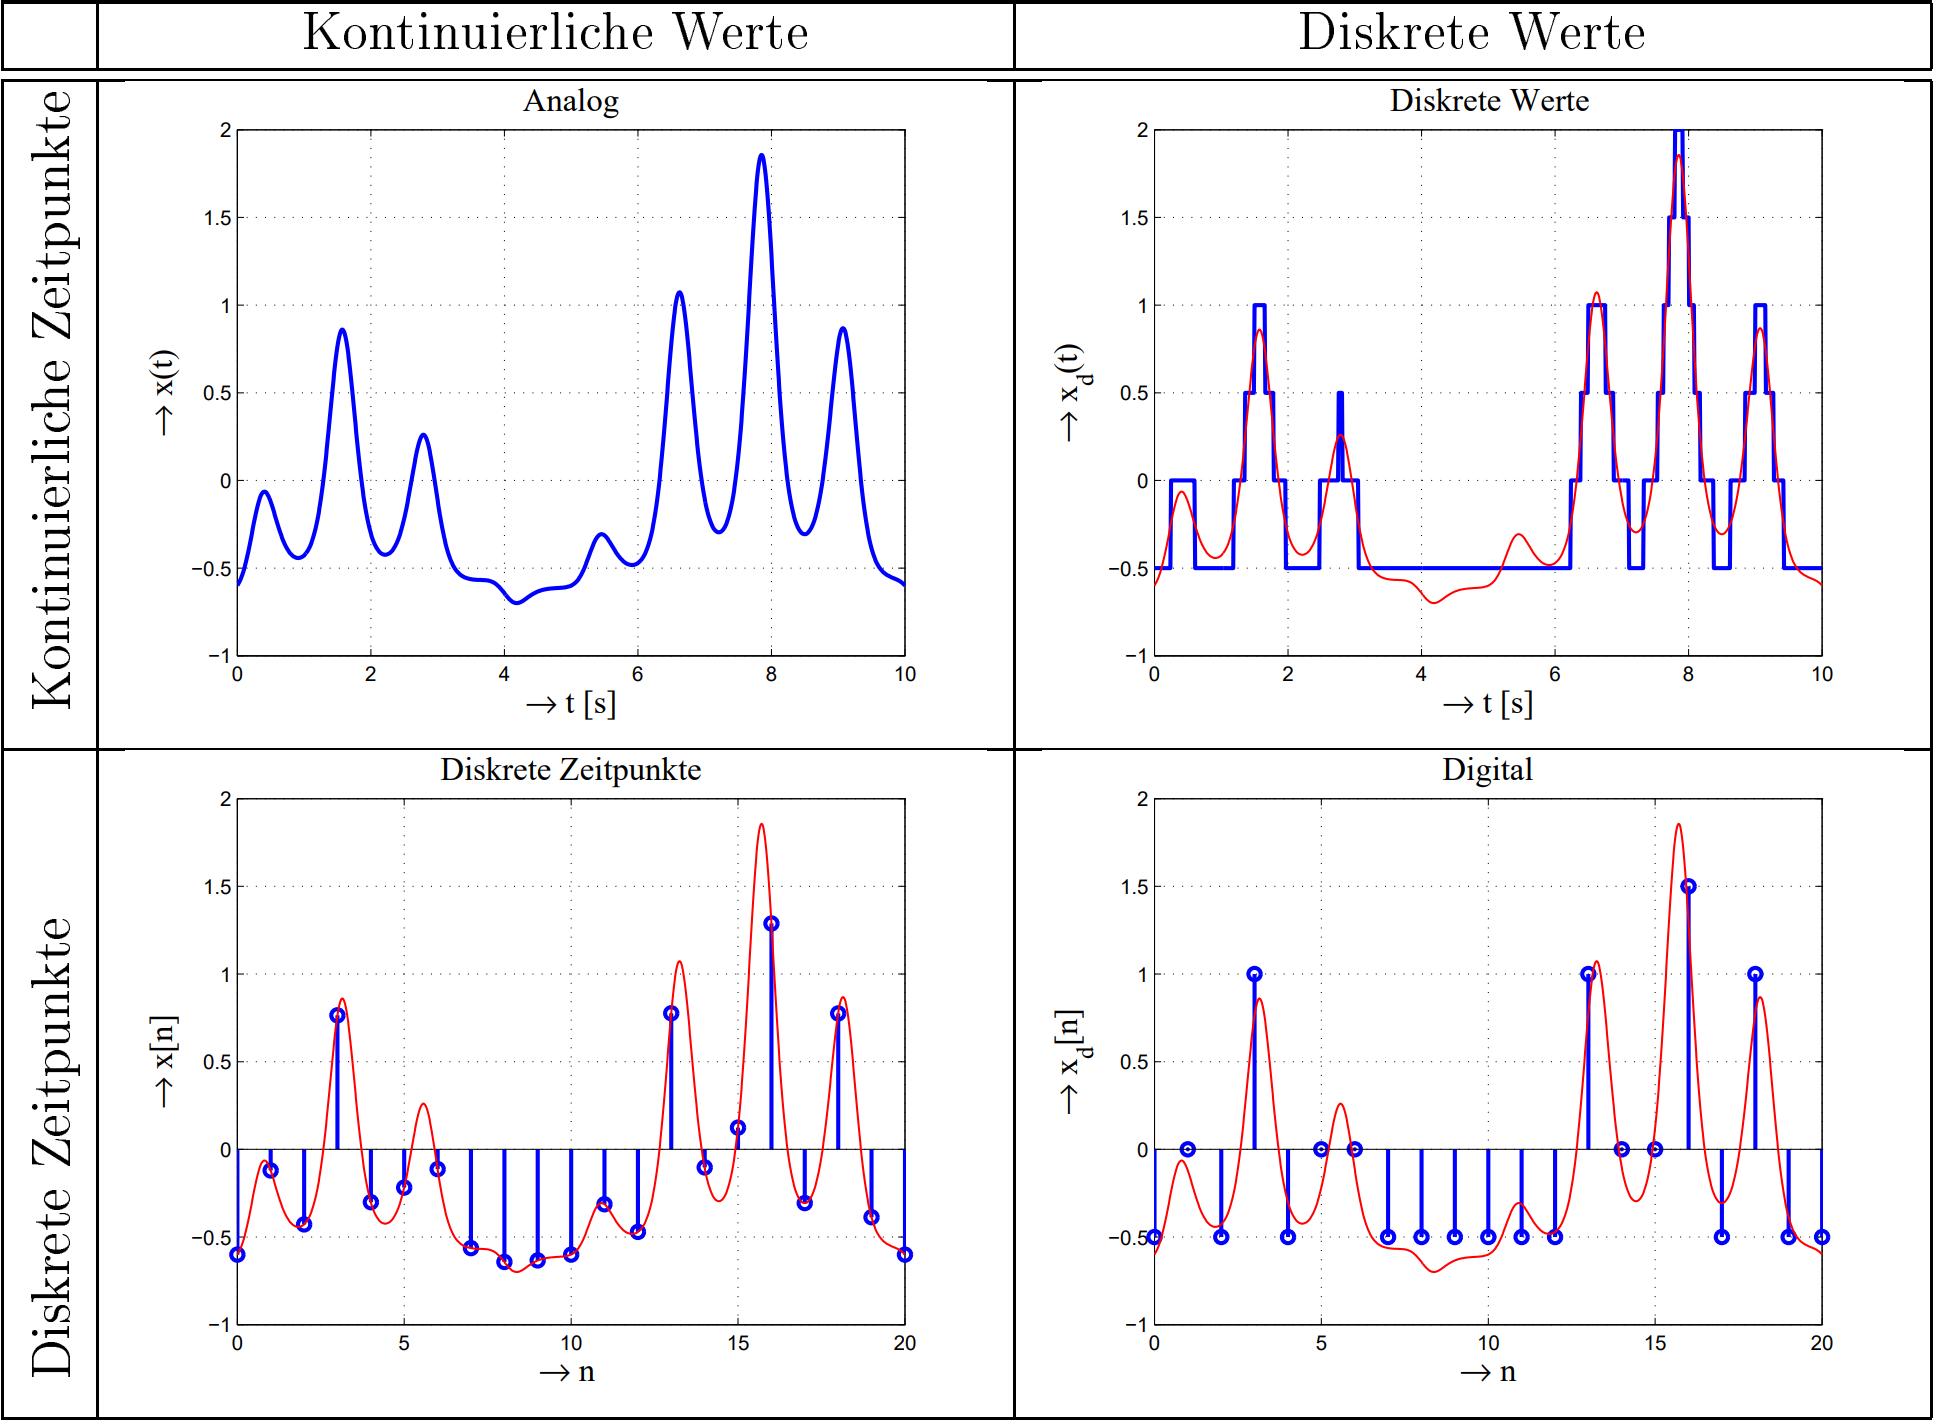
\includegraphics[width = 7cm]{img/Signalklassen.png}
  \subsection{weiter Unterteilungen}
    \begin{tabular}{|c|c|}
    Reell $\mathbb{R}$  &  Complex $\mathbb{C}$ \\
    Eindimensional & Mehrdimensional\\
    Stochastisch & Deterministisch \\
    Energiesignale & Leistungssignal \\
    \end{tabular}
\end{multicols}
\begin{tabular}{lll}
  Energiesiegnal Klasse 1 &
  Energiesiegnal Klasse 2a &
  Energiesiegnal Klasse 2b
\end{tabular}
 

\section{Mittelwerte}
\begin{tabular}{ccc}
  Linearer Mittelwert & Quadratischer Mittelwert & Effektivwert \tiny{(Quadratischer Mittelwert)}\\
  $ x_m = \bar{x} = x_0 = \frac{1}{T} 
  \int \limits _{-T/2}^{T/2} x(t) dt $ &
  $ x^2 = \frac{1}{T} \int \limits _{T/2}^{-T/2} x^2(t) dt $ &
  $ x^2 = \frac{1}{T} \int \limits _{T/2}^{-T/2} \sqrt{x^2(t)} dt $

\end{tabular} 




\end{document}
